\chapter*{Schoorl en Schoorldam}

\lettrine[lines=2, loversize=0.3, lraise=0]{\initfamily T}{oen } ik 11 was zijn we naar Schoorl verhuisd. In december 1939. Vlak voor de Duitsers kwamen.

Wij vonden het wel leuk om naar Schoorl te verhuizen maar voor m’n vader was het niet zo leuk. Hij was maagpati\"{e}nt geworden en kon het bedrijf niet meer doen. Hij had last van maagbloedingen. 

Ik vond het leuk om het duin in te gaan.


In december zijn we er gaan wonen en in het voorjaar kwamen de Duitsers. Ik weet nog goed dat mijn vader en ik uit bed waren gegaan. Het wemelde toen van de vliegtuigen. Na 5 dagen gaf Nederland zich over. Toen kwamen er ook Duitsers in Schoorl. 

\begin{figure}[h]
    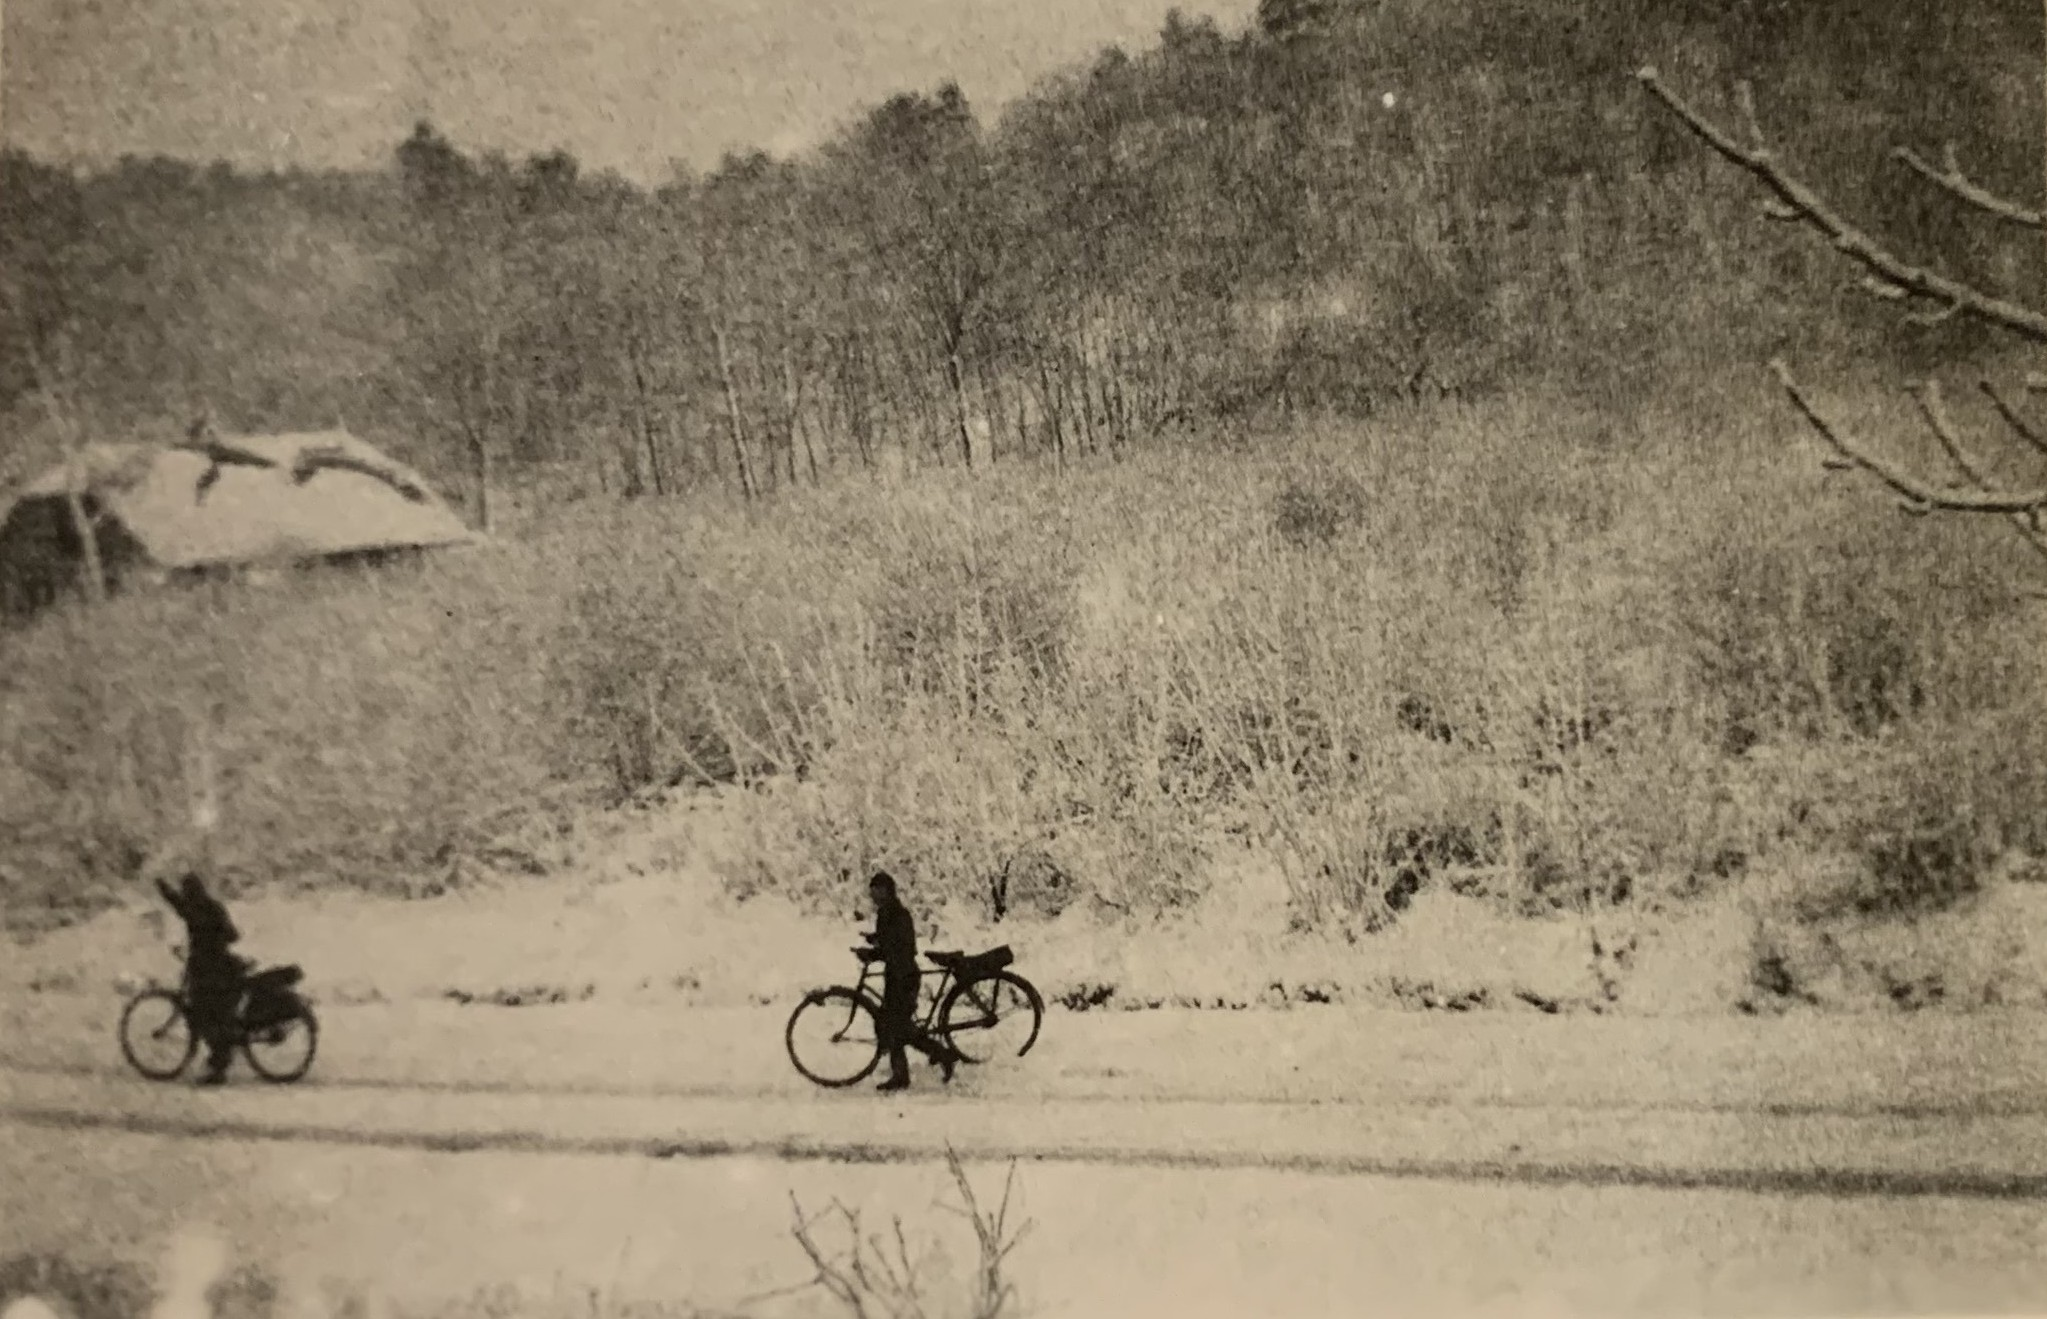
\includegraphics[width=1\textwidth]{image24}
    \caption{Kees en Tine gaan op de fiets naar school.}
\end{figure}

Ik herinner me dat opa Vlam vertelde dat hij met een Duitser had gepraat, dat was een boerenzoon, die moest in dienst. Dat was een goede Duitser zei opa. Die Duitsers zijn toen op de thee geweest. Toen zeiden wij dat moeten jullie maar niet meer doen.

Bert is toen ondergedoken. Eerst wisten we niet waar hij zat. Op een gegeven moment was hij 

ondergedoken in Noord-Holland. Toen zijn mijn moeder en tante Hidda op de fiets bij hem langs geweest. Bert kon daarna vrijstelling krijgen als hij aan de landbouwhogeschool ging studeren in Groningen. Daar heeft hij de oorlogsjaren op gezeten. 

Voor mij ging de school al die jaren gewoon door. Ik ging meestal met de fiets naar school.

Maar soms met de bus. Achter de bus zat een apart karretje dat stookten ze op turf en daar reed de bus op. Er zaten soms ook gewoon Duitsers in die keurig een kaartje kochten. Ik deed de huishoudkundige opleiding maar de laatste winter was er niks meer om mee te koken en ging de school ook dicht.

Soms als we naar school moesten fietsen lag er heel veel sneeuw. Dat werd toen natuurlijk niet opgeruimd alleen maar platgereden.

Aan het eind van de oorlog moesten we evacueren. Want ze waren bang voor landingen via het strand en collaboratie. Toen gingen we naar Schoorldam. Dat was heel gezellig. Bij opa en oma. Eerst sliep ik met Kees op zolder. Maar op een geven moment bleef tante Hidda op de boerderij en toen mocht ik in tante Hidda’s slaapkamer. Voor ons kinderen was het allemaal niet zo erg. In die tijd was er geen elektriciteit en werd de stal tijdens het melken verlicht met olielampjes. De reden was niet leuk maar het zag er zo gezellig uit!

\begin{figure}[h]
    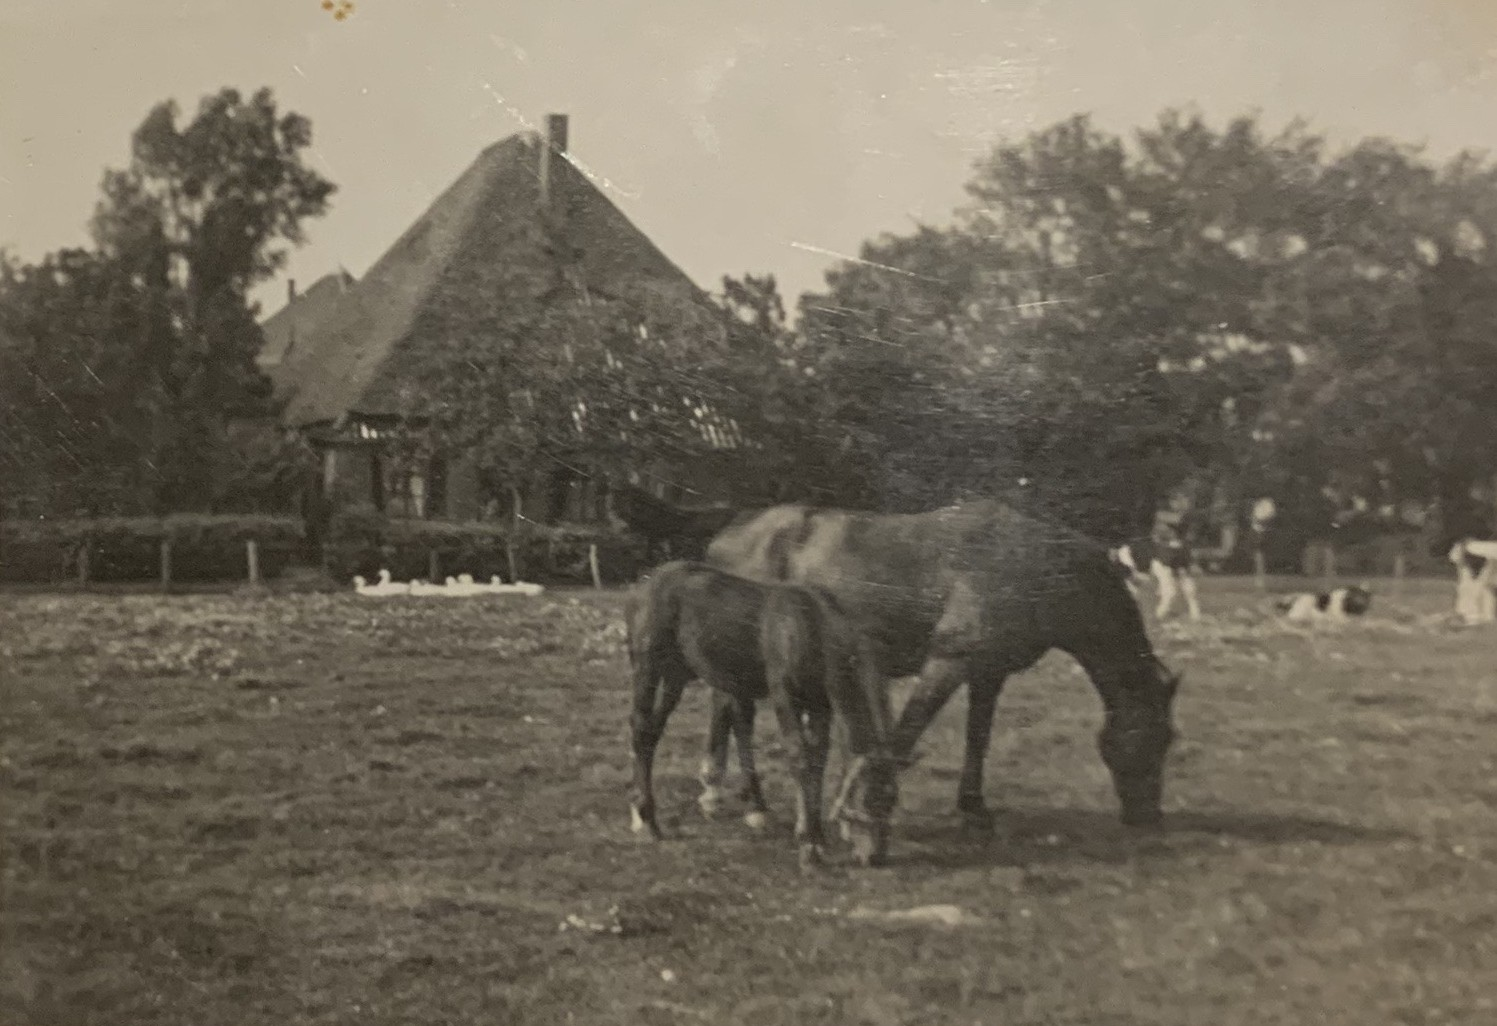
\includegraphics[width=1\textwidth]{image25}
    \caption{De boerderij op Schoorldam.}
\end{figure}

\begin{figure}[h]
    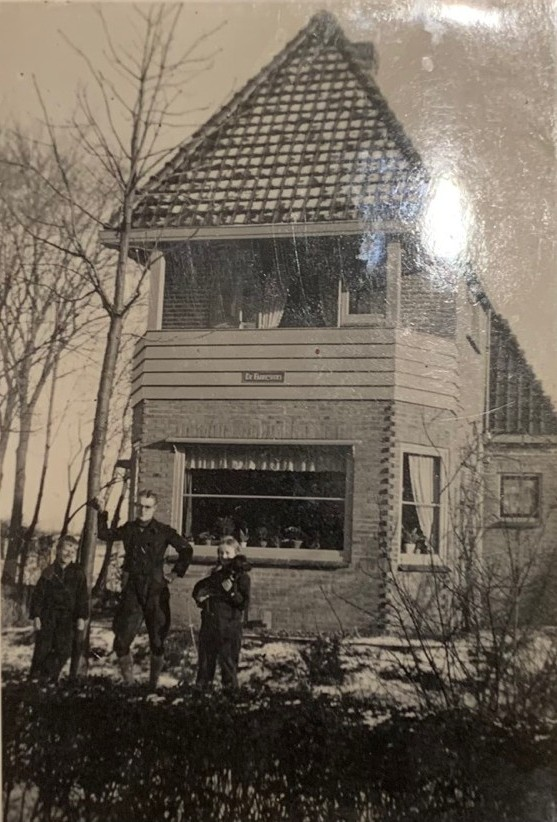
\includegraphics[width=0.9\textwidth]{image23}
    \caption{Het huis in Schoorl.}
\end{figure}

Mijn vader was gewoon thuis. Eens kwamen er ’s avonds een paar Duitse militairen in vol uniform en werd hij gecharterd om aan de Atlantikwall te werken. Hij moest daarbij helpen. Hij heeft er reuzepret gehad. Ze maakten alles zo langzaam en slecht mogelijk. 

Ook mijn beide opa’s konden gewoon thuis blijven, want ze hadden nuttige beroepen. De ene was boer op Schoorldam en de ander smid in Oudkarspel. 

Op een gegeven moment zei opa we gaan weer terug naar Schoorl. Eigenlijk mocht dat nog niet. Dat was voor de bevrijding maar de Duitsers waren al haast verslagen en ze lieten ons met rust toen we naar huis gingen.

Toen kwam de bevrijding. Dat hoorden we op de radio! Toen was iedereen blij en vrolijk. En moesten we allemaal weer een beetje de draad oppakken. 

In de oorlog was het een beetje saai. Er was helemaal niks te doen. Alles was dicht of verboden. Het enige wat er nog was de KJVO. De Kennemer jeugdgroep voor onthouders. Dat was opgezet door een leraar van de MULO. 

Dat was heel gezellig. Er werd elke week een gezellige avond georganiseerd met een lezing of we deden zelf dingen. En we zongen ook. In de winter hadden we dan een zangavond. En er werd toneel gespeeld.

We gingen kamperen met de KJVO op de Veluwe bij Doornspeijk. Dan gingen we om 4 uur s ochtend op de fiets van Schoorl naar Amsterdam om de eerste boot naar de Veluwe vanaf Amsterdam naar Harderwijk te kunnen pakken. En dan weer fietsten we daarna van Harderwijk naar Doornspeijk. We siepen in schaapskooien. Eentje voor de jongens en eentje voor ons. Dat was heel gezellig. Schuil organiseerde dat allemaal. Hij kende daar boeren. Je kon je bij de pomp wassen met koud water. Er was geen toilet maar een kuil buiten in het bos. Dat ging ook best. We wandelden en fietsen veel. Dankzij opa hadden wij ook fietsen. Er was ook een Joodse jongen mee die eigenlijk was ondergedoken. Dat vond ik altijd wel eng als we Duitsers tegenkwamen maar het is gelukkig allemaal goed gegaan. 